%%%%%%%%%%%%%%%%%%%%%%%%%%%%%%%%%%%%%%%%%
% Beamer Presentation
% LaTeX Template
% Version 1.0 (10/11/12)
%
% This template has been downloaded from:
% http://www.LaTeXTemplates.com
%
% License:
% CC BY-NC-SA 3.0 (http://creativecommons.org/licenses/by-nc-sa/3.0/)
%
%%%%%%%%%%%%%%%%%%%%%%%%%%%%%%%%%%%%%%%%%

%----------------------------------------------------------------------------------------
%	PACKAGES AND THEMES
%----------------------------------------------------------------------------------------

\documentclass{beamer}

\mode<presentation> {

% The Beamer class comes with a number of default slide themes
% which change the colors and layouts of slides. Below this is a list
% of all the themes, uncomment each in turn to see what they look like.

%\usetheme{default}
%\usetheme{AnnArbor}
%\usetheme{Antibes}
%\usetheme{Bergen}
%\usetheme{Berkeley}
%\usetheme{Berlin}
%\usetheme{Boadilla}
%\usetheme{CambridgeUS}
%\usetheme{Copenhagen}
%\usetheme{Darmstadt}
%\usetheme{Dresden}
%\usetheme{Frankfurt}
%\usetheme{Goettingen}
%\usetheme{Hannover}
%\usetheme{Ilmenau}
%\usetheme{JuanLesPins}
%\usetheme{Luebeck}
%\usetheme{Madrid}
%\usetheme{Malmoe}
%\usetheme{Marburg}
\usetheme{Montpellier}
%\usetheme{PaloAlto}
%\usetheme{Pittsburgh}
%\usetheme{Rochester}
%\usetheme{Singapore}
%\usetheme{Szeged}
%\usetheme{Warsaw}

% As well as themes, the Beamer class has a number of color themes
% for any slide theme. Uncomment each of these in turn to see how it
% changes the colors of your current slide theme.

%\usecolortheme{albatross}
%\usecolortheme{beaver}
%\usecolortheme{beetle}
%\usecolortheme{crane}
\usecolortheme{dolphin}
%\usecolortheme{dove}
%\usecolortheme{fly}
%\usecolortheme{lily}
%\usecolortheme{orchid}
%\usecolortheme{rose}
%\usecolortheme{seagull}
%\usecolortheme{seahorse}
%\usecolortheme{whale}
%\usecolortheme{wolverine}

%\setbeamertemplate{footline} % To remove the footer line in all slides uncomment this line
%\setbeamertemplate{footline}[page number] % To replace the footer line in all slides with a simple slide count uncomment this line

%\setbeamertemplate{navigation symbols}{} % To remove the navigation symbols from the bottom of all slides uncomment this line
}

\usepackage{graphicx} % Allows including images
\usepackage{booktabs} % Allows the use of \toprule, \midrule and \bottomrule in tables
\usepackage{listings}
\usepackage{color}

\usepackage{minted}
%\usepackage[utf8]{inputenc}
\usepackage[english]{babel}

\definecolor{darkgray}{gray}{0.1}
\definecolor{lbcolor}{rgb}{0.9,0.9,0.9}
\definecolor{mauve}{rgb}{0.48,0,0.72}

\lstset{
  language=C++,                   % choose the language of the code
  backgroundcolor=\color{white},  % choose the background color. You must add \usepackage{color}
  basicstyle=\ttfamily,
  numberstyle=\color{mauve}\ttfamily,
  keywordstyle=\color{blue}\ttfamily,
  stringstyle=\color{red}\ttfamily,
  commentstyle=\color{green}\ttfamily,
  frame=single,
  showspaces=false,               % show spaces adding particular underscores
  showstringspaces=false,         % underline spaces within strings
  showtabs=false,                 % show tabs within strings adding particular underscores
  tabsize=2,                      % sets default tabsize to 2 spaces
  captionpos=b,                   % sets the caption-position to bottom
  breaklines=false,                % sets automatic line breaking
  breakatwhitespace=false,         % sets if automatic breaks should only happen at whitespace
  title=\lstname,                 % show the filename of files included with \lstinputlisting;
}

%----------------------------------------------------------------------------------------
%	TITLE PAGE
%----------------------------------------------------------------------------------------

\title[COIN OR]{COIN OR Project \\* (Computational Infrastructure for Operations Research)} % The short title appears at the bottom of every slide, the full title is only on the title page

\author{Dimitris Dimou \\* Alexandros Zigouris} % Your name
\institute[UP] % Your institution as it will appear on the bottom of every slide, may be shorthand to save space
{
University of Patras \\ % Your institution for the title page
\medskip
\textit{mijuomij@gmail.com} % Your email address
}
\date{\today} % Date, can be changed to a custom date

\begin{document}

\begin{frame}
\titlepage % Print the title page as the first slide
\end{frame}

\begin{frame}
\frametitle{Overview} % Table of contents slide, comment this block out to remove it
\tableofcontents % Throughout your presentation, if you choose to use \section{} and \subsection{} commands, these will automatically be printed on this slide as an overview of your presentation
\end{frame}

%----------------------------------------------------------------------------------------
%	PRESENTATION SLIDES
%----------------------------------------------------------------------------------------

%------------------------------------------------
\section{CLP for Linear Programming} % Sections can be created in order to organize your presentation into discrete blocks, all sections and subsections are automatically printed in the table of contents as an overview of the talk

%------------------------------------------------

\subsection{Installation} % A subsection can be created just before a set of slides with a common theme to further break down your presentation into chunks


\begin{frame}
  \frametitle{Installation}
  \begin{enumerate}
    \item svn co https://projects.coin-or.org/svn/Clp/stable/1.16 coin-Clp
    \item cd coin-Clp
    \item ./configure -C
    \item make 
    \item make test
    \item make install
    \item make doxydoc
  \end{enumerate}
\end{frame}

%------------------------------------------------

\subsection{Overeview}

\begin{frame}
\frametitle{Background}
Clp is written in C++ and is released as open source code under the ​Eclipse Public License (EPL). It is available from the ​COIN-OR initiative. The code is written primarily by John J. Forrest, now retired from IBM Research. The project is currently managed by John Forrest, ​Julian Hall, and the rest of the ​Clp team. \\*
The latest stable version is 1.16.
\end{frame}

\begin{frame}
 	\frametitle{Basic model classes}
  The top three levels of the hierarchy are depicted in the figure below. The first two levels (i.e. ClpModel, ClpSimplex, ClpInterior) contain all the problem data which define a model (that is, a problem instance). The third level contains most of the algorithmic aspects of CLP.
  \begin{figure}
  	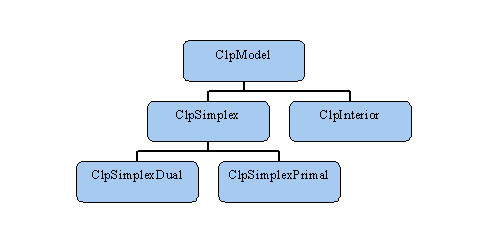
\includegraphics[width=0.8\linewidth]{clpbasicmodelhier}
  \end{figure}
\end{frame}

\begin{frame}[fragile]
  \frametitle{Load model}
  \begin{itemize}
    \item Load from matrix
  \end{itemize}
  \begin{minted}[fontsize=\scriptsize]{cpp}
  void ClpModel::loadProblem (const ClpMatrixBase &matrix, 
                              const double *collb, 
                              const double *colub, 
                              const double *obj, 
                              const double *rowlb, 
                              const double *rowub, 
                              const double *rowObjective = NULL)
  \end{minted}
  \begin{itemize}
    \item{\footnotesize} Load from MPS file
  \end{itemize}
  \begin{minted}[fontsize=\scriptsize]{cpp}
  int ClpModel::readMps (const char *filename, 
                         bool keepNames = false, 
                         bool ignoreErrors = false)   
  \end{minted}
  \begin{itemize}
    \item Load from GMPL file
  \end{itemize}
  \begin{minted}[fontsize=\scriptsize]{cpp}
  int ClpModel::readGMPL (const char *filename, 
                          const char *dataName, 
                          bool keepNames = false)     
  \end{minted}
\end{frame}

\begin{frame}[fragile]
  \frametitle{MPS format}
  \begin{lstlisting}[basicstyle=\tiny]
  NAME          DOVETAIL  
ROWS
 N  obj
 L  c1    
 L  c2
 L  c3
 L  c4
COLUMNS
    MARK0000  'MARKER'                 'INTORG'
    x1        obj                  3   c1                   1
    x1        c2                   3   c3                   1
    x2        obj                  2   c1                   1
    x2        c2                   1   c4                   1
    MARK0001  'MARKER'                 'INTEND'
RHS
    RHS       c1                   9   c2                  18
    RHS       c3                   7   c4                   6
BOUNDS
 LO BND       x1                   0
 LO BND       x2                   0
ENDATA
 \end{lstlisting}
\end{frame}

%------------------------------------------------

\subsection{Usage}
{
\setbeamercolor{background canvas}{bg=darkgray}
\begin{frame}[fragile]
	\usemintedstyle{monokai}
	\inputminted{cpp}{examples/simplex_minimum.cpp}
\end{frame}
}

\newcommand{\itab}[1]{\hspace{0em}\rlap{#1}}
\newcommand{\tab}[1]{\hspace{.15\textwidth}\rlap{#1}}

\begin{frame}
 \frametitle{Solution inspection}
 \begin{itemize}
  \item \itab{double *} \tab{model.primalColumnSolution();}
  \item \itab{double *} \tab{model.primalRowSolution();}
  \item \itab{bool} 	\tab{model.isProvenOptimal();}
  \item \itab{bool} 	\tab{model.isProvenPrimalInfeasible();}
  \item \itab{bool} 	\tab{model.isProvenDualInfeasible();}
  \item \itab{bool} 	\tab{model.isIterationLimitReached();}
 \end{itemize}
\end{frame}

\begin{frame}
  \frametitle{Other useful methods}
  \begin{block}{Set methods}
    \begin{itemize}
    \item model.setMaximumIterations(int value);
    \item model.setMaximumSeconds(double value);
    \item model.setDualBound(double value);
    \item model.setOptimizationDirection(double value);
    \end{itemize}
  \end{block}
 \begin{block}{Get methods}
    \begin{itemize}
    \item model.numberRows();
    \item model.numberColumns();
    \item model.objectiveValue();
    \item model.objective();
    \end{itemize}
 \end{block}
\end{frame}

\begin{frame}
  \frametitle{Pivot choices}
  \begin{itemize}
  \item ClpPrimalColumnPivot
    \begin{itemize}
    \item ClpPrimalColumnSteepest
    \item ClpPrimalColumnDantzig
    \end{itemize}
  \item ClpDualRowSteepest
    \begin{itemize}
    \item ClpDualRowDantzig
    \item ClpDualRowPivot
    \end{itemize}
  \end{itemize}
\end{frame}
%------------------------------------------------

\subsection{Basic examples}

\begin{frame}
\frametitle{Bullet Points}
\end{frame}

%------------------------------------------------

\end{document} 